\documentclass{alex_hü}

\name{Alexander Helbok}
\course{PS Vorbereitungskurs Mathematik}
\hwnumber{2}

\begin{document}
	\renewcommand{\labelenumi}{\arabic{enumi})}
	
	
	\section*{1. Verlauf von Funktionen}
	\begin{enumerate}
		\item Gaußverteilung: $ f(x) = exp(−x^2) $ für $ x \in \left[−2 : 2\right]  $
		\begin{multicols}{2}
		\begin{tikzpicture}
			\begin{axis}[
				width=207pt,
				height=207pt,
				axis lines=center,
				x axis line style={Stealth-Stealth},
				xmin=-2.9,xmax=2.9,ymin=0,ymax=1.24,
				xlabel style={below},
				xtick distance=1,
				ytick distance=0.25,
				tick label style={font=\small},
				xlabel=$x$,
				ylabel=$y$,
				grid=major,
				grid style={thin,densely dotted,black!20},
				%legend columns=2,
				legend style={at={(axis description cs:1,0.35)},anchor=east}]
				\addplot [thick, red, mark=square, only marks]
				plot coordinates {
					(-2.0,0.02)(-1.75,0.05)(-1.5,0.11)
					(-1.25,0.21)(-1.0,0.37)(-0.75,0.57)
					(-0.5,0.78)(-0.25,0.94)(0.0,1.0)
					(0.25,0.94)(0.5,0.78)(0.75,0.57)
					(1.0,0.37)(1.25,0.21)(1.5,0.11)
					(1.75,0.05)(2.0,0.02)
				};	
				\addplot [smooth, thick, red, domain = -3:3] {e^-x^2)};
			\end{axis}
		\end{tikzpicture}\\
		\columnbreak
		\begin{multicols}{2}
			\begin{align*}
				f\left(-2\right) &= 0.02 \\
				f\left(-1.75\right) &= 0.05 \\
				f\left(-1.5\right) &= 0.11 \\
				f\left(-1.25\right) &= 0.21 \\
				f\left(-1\right) &= 0.37 \\
				f\left(-0.75\right) &= 0.57 \\
				f\left(-0.5\right) &= 0.78 \\
				f\left(-0.25\right) &= 0.94 \\
			\end{align*}
			\columnbreak
			\begin{align*}\\
				f\left(0\right) &= 1 \\
				f\left(0.25\right) &= 0.94 \\
				f\left(0.5\right) &= 0.78 \\
				f\left(0.75\right) &= 0.57 \\
				f\left(1\right) &= 0.37 \\
				f\left(1.25\right) &= 0.21 \\
				f\left(1.5\right) &= 0.11 \\
				f\left(1.75\right) &= 0.05 \\
				f\left(2\right) &= 0.02 \\
			\end{align*}
		\end{multicols}
		
	\end{multicols}
		\item  Lorentzkurve: $ f(x) = 1/1 + x^2 $ für $  x \in \left[−2 : 2\right] $
		\begin{multicols}{2}
			\begin{tikzpicture}
				\begin{axis}[
					width=207pt,
					height=207pt,
					axis lines=center,
					x axis line style={Stealth-Stealth},
					xmin=-2.9,xmax=2.9,ymin=0,ymax=1.24,
					xlabel style={below},
					xtick distance=1,
					ytick distance=0.25,
					tick label style={font=\small},
					xlabel=$x$,
					ylabel=$y$,
					grid=major,
					grid style={thin,densely dotted,black!20},
					%legend columns=2,
					legend style={at={(axis description cs:1,0.35)},anchor=east}]
					\addplot [thick, red, mark=square, only marks]
					plot coordinates {
						(-2.0,0.2)(-1.75,0.25)(-1.5,0.31)
						(-1.25,0.39)(-1.0,0.5)(-0.75,0.64)
						(-0.5,0.8)(-0.25,0.94)(0.0,1.0)
						(0.25,0.94)(0.5,0.8)(0.75,0.64)
						(1.0,0.5)(1.25,0.39)(1.5,0.31)
						(1.75,0.25)(2.0,0.2)
					};	
					\addplot [smooth, thick, red] {1/(1 + x^2)};
				\end{axis}
			\end{tikzpicture}\\
			\columnbreak
			\begin{multicols}{2}
				\begin{align*}
					f\left(-2\right) &= 0.2 \\
					f\left(-1.75\right) &= 0.25 \\
					f\left(-1.5\right) &= 0.31 \\
					f\left(-1.25\right) &= 0.39 \\
					f\left(-1\right) &= 0.5 \\
					f\left(-0.75\right) &= 0.64 \\
					f\left(-0.5\right) &= 0.8 \\
					f\left(-0.25\right) &= 0.94 \\
				\end{align*}
			\columnbreak
				\begin{align*}\\
					f\left(0\right) &= 1 \\
					f\left(0.25\right) &= 0.94 \\
					f\left(0.5\right) &= 0.8 \\
					f\left(0.75\right) &= 0.64 \\
					f\left(1\right) &= 0.5 \\
					f\left(1.25\right) &= 0.39 \\
					f\left(1.5\right) &= 0.31 \\
					f\left(1.75\right) &= 0.25 \\
					f\left(2\right) &= 0.2 
				\end{align*}
			\end{multicols}
			
		\end{multicols}
		\newpage
		\item Bose-Einstein Verteilung: $ f(x) = 1/(e^x − 1) $ für $ x \in \left[0 : 4\right] $
		\begin{multicols}{2}
			\begin{tikzpicture}
				\begin{axis}[
					width=207pt,
					height=207pt,
					axis lines=center,
					axis line style={Stealth-Stealth},
					xmin=-4.9,xmax=4.9,ymin=-6.9,ymax=6.9,
					xlabel style={below},
					xtick distance=1,
					ytick distance=1,
					xlabel=$x$,
					ylabel=$y$,
					tick label style={font=\tiny},
					grid=major,
					grid style={thin,densely dotted,black!20},
					%legend columns=2,
					legend style={at={(axis description cs:1,0.35)},anchor=east}]
					\addplot [thick, red, mark=square, only marks]
					plot coordinates {
						(-4.0,-1.02)(-3.0,-1.05)
						(-2.0,-1.16)(-1.5,-1.29)
						(-1.0,-1.58)(-0.45,-2.54)
					};	
					\addplot [thick, red, mark=square, only marks]
					plot coordinates {
						(0.3,3.52)(0.45,1.54)(0.75,0.9)(1.0,0.58)(1.5,0.29)
						(2.0,0.16)(3.0,0.05)
						(4.0,0.02)
					};	
					\addplot [smooth, thick, red, domain = 0.1:6] {1/(e^x - 1)};
					\addplot [smooth, thick, red, domain = -6:-0.1] {1/(e^x - 1)};
				\end{axis}
			\end{tikzpicture}\\
			\columnbreak
			\begin{multicols}{2}
				\begin{align*}
					f\left(-4\right) &= -1.02 \\
					f\left(-3\right) &= -1.05 \\
					f\left(-2\right) &= -1.16 \\
					f\left(-1.5\right) &= -1.29 \\
					f\left(-1\right) &= -1.58 \\
					f\left(-0.75\right) &= -1.9 \\
					f\left(-0.5\right) &= -2.54 \\
					f\left(-0.25\right) &= -4.52 \\
				\end{align*}
				\columnbreak
				\begin{align*}\\
					f\left(0\right) &= \text{nicht definiert} \\
					f\left(0.25\right) &= 3.52 \\
					f\left(0.5\right) &= 1.54 \\
					f\left(0.75\right) &= 0.9 \\
					f\left(1\right) &= 0.58 \\
					f\left(1.5\right) &= 0.29 \\
					f\left(2\right) &= 0.16 \\
					f\left(3\right) &= 0.05 \\
					f\left(4\right) &= 0.02 \\
				\end{align*}
			\end{multicols}
		\end{multicols}
		\item  Sinc-Funktion: $ f(x) = \sin(x) / x \text{ für } x \in [−10 : 10] $
		\begin{multicols}{2}
			\begin{tikzpicture}
				\begin{axis}[
					width=207pt,
					height=207pt,
					axis lines=center,
					axis line style={Stealth-Stealth},
					xmin=-10.9,xmax=10.9,ymin=-0.7,ymax=1.2,
					xlabel style={below},
					xtick distance=5,
					ytick distance=0.25,
					xlabel=$x$,
					ylabel=$y$,
					tick label style={font=\small},
					grid=major,
					grid style={thin,densely dotted,black!20},
					%legend columns=2,
					legend style={at={(axis description cs:1,0.35)},anchor=east}]
					\addplot [thick, red, mark=square, only marks]
					plot coordinates {
						(-10,-0.05)(-9,0.05)(-8,0.12)(-7,0.09)
						(-6,-0.05)(-5,-0.19)(-4,-0.19)
						(-3,0.05)(-2,0.45)(-1,0.84)(0,1)
						(1,0.84)(2,0.45)(3,0.05)
						(4,-0.19)(5,-0.19)(6,-0.05)
						(7,0.09)(8,0.12)(9,0.05)
						(10,-0.05)
					};	
					\addplot [smooth, thick, red, domain = -11:11] {sin(deg(x))/x};
				\end{axis}
			\end{tikzpicture}\\
			\columnbreak
			\begin{multicols}{2}
				\begin{align*}
					f\left(-10\right) &= -0.05 \\
					f\left(-9\right) &= 0.05 \\
					f\left(-8\right) &= 0.12 \\
					f\left(-7\right) &= 0.09 \\
					f\left(-6\right) &= -0.05 \\
					f\left(-5\right) &= -0.19 \\
					f\left(-4\right) &= -0.19 \\
					f\left(-3\right) &= 0.05 \\
					f\left(-2\right) &= 0.45 \\
					f\left(-1\right) &= 0.84 \\
				\end{align*}
				\columnbreak
				\begin{align*}\\
					f\left(0\right) &= 1 \\
					f\left(1\right) &= 0.84 \\
					f\left(2\right) &= 0.45 \\
					f\left(3\right) &= 0.05 \\
					f\left(4\right) &= -0.19 \\
					f\left(5\right) &= -0.19 \\
					f\left(6\right) &= -0.05 \\
					f\left(7\right) &= 0.09 \\
					f\left(8\right) &= 0.12 \\
					f\left(9\right) &= 0.05 \\
					f\left(10\right) &= -0.05 \\
				\end{align*}
			\end{multicols}
		\end{multicols}
		\newpage
		\item $ f(x) = x^x \text{ für } x \in [0 : 3] $
		\begin{multicols}{2}
			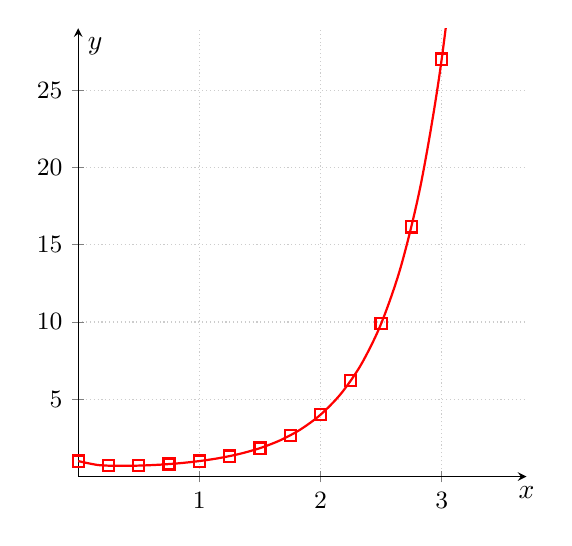
\begin{tikzpicture}
				\begin{axis}[
					width=207pt,
					height=207pt,
					axis lines=center,
%					axis line style={Stealth-Stealth},
					xmin=0,xmax=3.7,ymin=0,ymax=29,
					xlabel style={below},
					xtick distance=1,
					ytick distance=5,
					xlabel=$x$,
					ylabel=$y$,
					tick label style={font=\small},
					grid=major,
					grid style={thin,densely dotted,black!20},
					%legend columns=2,
					legend style={at={(axis description cs:1,0.35)},anchor=east}]
					\addplot [thick, red, mark=square, only marks]
					plot coordinates {
						(0.0,1.0)(0.25,0.71)(0.5,0.71)
						(0.75,0.81)(1.0,1.0)(1.25,1.32)
						(1.5,1.84)(1.75,2.66)(2.0,4.0)
						(2.25,6.2)(2.5,9.88)(2.75,16.15)
						(3.0,27.0)
					};	
					\addplot [smooth, thick, red, domain = 0.00001:4] {x^x};
				\end{axis}
			\end{tikzpicture}\\
			\columnbreak
			\begin{multicols}{2}
				\begin{align*}
					f\left(-10\right) &= -0.05 \\
					f\left(-9\right) &= 0.05 \\
					f\left(-8\right) &= 0.12 \\
					f\left(-7\right) &= 0.09 \\
					f\left(-6\right) &= -0.05 \\
					f\left(-5\right) &= -0.19 \\
					f\left(-4\right) &= -0.19 \\
					f\left(-3\right) &= 0.05 \\
					f\left(-2\right) &= 0.45 \\
					f\left(-1\right) &= 0.84 \\
				\end{align*}
				\columnbreak
				\begin{align*}\\
					f\left(0\right) &= 1 \\
					f\left(1\right) &= 0.84 \\
					f\left(2\right) &= 0.45 \\
					f\left(3\right) &= 0.05 \\
					f\left(4\right) &= -0.19 \\
					f\left(5\right) &= -0.19 \\
					f\left(6\right) &= -0.05 \\
					f\left(7\right) &= 0.09 \\
					f\left(8\right) &= 0.12 \\
					f\left(9\right) &= 0.05 \\
					f\left(10\right) &= -0.05 \\
				\end{align*}
			\end{multicols}
		\end{multicols}
	\end{enumerate}
	
%	\section*{3. Analyse einer quadratischen Funktion}

\end{document}